%%%%%%%%%%%%%%%%%%%%%%%%%%%%%%%%%%%%%%%%%%%%%%%%%%%%%%%%%%%%%%%%
% %
% Seth Cram %
% ECE351 Section 53 %
% Lab 8 %
% Due 03/15/2022 %
% Any other necessary information needed to navigate the file %
%
%
% %
%%%%%%%%%%%%%%%%%%%%%%%%%%%%%%%%%%%%%%%%%%%%%%%%%%%%%%%%%%%%%%%%
%%%%%%%%%%%%%%%%%%%%%%%%%%%%%%%%%%%%%%%%%%%
%%% DOCUMENT PREAMBLE %%%
\documentclass[12pt]{report}
\usepackage[english]{babel}
%\usepackage{natbib}
\usepackage{url}
\usepackage[utf8x]{inputenc}
\usepackage{amsmath}
\usepackage{graphicx}
\graphicspath{{images/}}
\usepackage{parskip}
\usepackage{fancyhdr}
\usepackage{vmargin}
\usepackage{listings}
\usepackage{hyperref}
\usepackage{xcolor}
\usepackage{verbatim}
\usepackage{listings}

\definecolor{codegreen}{rgb}{0,0.6,0}
\definecolor{codegray}{rgb}{0.5,0.5,0.5}
\definecolor{codeblue}{rgb}{0,0,0.95}
\definecolor{backcolour}{rgb}{0.95,0.95,0.92}

\begin{comment} %have to use verbatim package for this

\section{Personal Notes}
            


\end{comment}

\lstdefinestyle{mystyle}{
    backgroundcolor=\color{backcolour},   
    commentstyle=\color{codegreen},
    keywordstyle=\color{codeblue},
    numberstyle=\tiny\color{codegray},
    stringstyle=\color{codegreen},
    basicstyle=\ttfamily\footnotesize,
    breakatwhitespace=false,         
    breaklines=true,                 
    captionpos=b,                    
    keepspaces=true,                 
    numbers=left,                    
    numbersep=5pt,                  
    showspaces=false,                
    showstringspaces=false,
    showtabs=false,                  
    tabsize=2
}
 
\lstset{style=mystyle}

\setmarginsrb{3 cm}{2.5 cm}{3 cm}{2.5 cm}{1 cm}{1.5 cm}{1 cm}{1.5 cm}

\title{Lab 8}		%TITLE						
% Title
\author{ Seth Cram}						
% Author
\date{03/15/2022}
% Date

\makeatletter
\let\thetitle\@title
\let\theauthor\@author
\let\thedate\@date
\makeatother

\pagestyle{fancy}
\fancyhf{}
\rhead{\theauthor}
\lhead{\thetitle}
\cfoot{\thepage}
%%%%%%%%%%%%%%%%%%%%%%%%%%%%%%%%%%%%%%%%%%%%
\begin{document}

%%%%%%%%%%%%%%%%%%%%%%%%%%%%%%%%%%%%%%%%%%%%%%%%%%%%%%%%%%%%%%%%%%%%%%%%%%%%%%%%%%%%%%%%%

\begin{titlepage}
	\centering
    \vspace*{0.5 cm}
   % \includegraphics[scale = 0.075]{bsulogo.png}\\[1.0 cm]	% University Logo
\begin{center}    \textsc{\Large   ECE 351 - 53 }\\[2.0 cm]	\end{center}% University Name
	\textsc{\Large Fourier Series Approximation of a Square Wave }\\[.5 cm]				% Course Code
	\rule{\linewidth}{0.2 mm} \\[0.4 cm]
	{ \huge \bfseries \thetitle}\\
	\rule{\linewidth}{0.2 mm} \\[1.5 cm]
	
	\begin{minipage}{0.4\textwidth}
		\begin{flushleft} \large
		%	\emph{Submitted To:}\\
		%	Name\\
          % Affiliation\\
           %contact info\\
			\end{flushleft}
			\end{minipage}~
			\begin{minipage}{0.4\textwidth}
            
			\begin{flushright} \large
			\emph{Submitted By :} \\
			Seth Cram  
		\end{flushright}
           
	\end{minipage}\\[2 cm]
	
\end{titlepage}

%%%%%%%%%%%%%%%%%%%%%%%%%%%%%%%%%%%%%%%%%%%%%%%%%%%%%%%%%%%%%%%%%%%%%%%%%%%%%%%%%%%%%%%%%

\tableofcontents
\pagebreak

%%%%%%%%%%%%%%%%%%%%%%%%%%%%%%%%%%%%%%%%%%%%%%%%%%%%%%%%%%%%%%%%%%%%%%%%%%%%%%%%%%%%%%%%%
\renewcommand{\thesection}{\arabic{section}}

\section{Introduction}

The goal of lab 8 is to use Fourier Series to approximate periodic time-domain signals using Python loops in the Spyder IDE.

\section{Equations}
    \begin{equation}
       x(t) = \frac{1}{2}a_0 + \sum_{k=1}^{\infty} a_k*cos(kw_0t) + b_k*sin(kw_0t) = \sum_{k=1}^{\infty} \frac{2}{k\pi}(1-cos(k\pi))sin(kw_0t)
    \end{equation}

    \begin{equation}
        a_k = \frac{2}{T} * \int_{0}^{T} x(t)*cos(kw_0t) \,dt = 0
    \end{equation}
    
    \begin{equation}
        b_k = \frac{2}{T} * \int_{0}^{T} x(t)*sin(kw_0t) \,dt = \frac{2}{k\pi}(1-cos(k\pi))
    \end{equation}
 
     \begin{equation}
        a_0 = 0
    \end{equation}
    
    \begin{equation}
        a_1 = 0
    \end{equation}
    
    \begin{equation}
        b_1 =  0.63662
    \end{equation}
    
    \begin{equation}
        b_2 =  0
    \end{equation}
    
    \begin{equation}
        b_3 =  0.2122
    \end{equation}
    
\section{Methodology}

%This section will describe how you went about solving the lab. Make sure you go into detail about any method you used. %Include coding samples here if necessary. This is also where you would include necessary derivations. An example of %inserting code into the report is given. Do not go overboard on inserting code into your report, only use whats %absolutely necessary to illustrate your point.

    \paragraph{} First, I attempted to do the prelab. With the TA's help, I was successful. We hadn't fully covered the basics of Fourier transforms in-class yet, so it was fairly difficult. Now that I had the derived equations for $a_k$, $b_k$, and x(t), I was ready to start the lab. 
    
    \paragraph{} Then, I input both my expression for $a_k$ and $b_k$ into Spyder. I manually changed the k-value to calculate $a_0$, $a_1$, $b_1$, $b_2$, and $b_3$. I made sure to print these values out to the console and attached them to the Appendix in the report. 
    
    \paragraph{} I then detailed out a simple function to calculate x(t). I passed in t, T, and N as arguments to my function for re-usability purposes. T represented the period and N the number of iterations. Within this function I used the x(t) equation derived in the prelab to calculate and sum the value of x(t) for each time passed in as t. Returning this array as x(t), I was able to plot the functions with little trouble.
    
\section{Results}

%This section will go over the results of the lab. Use this area to describe %if the lab worked as expected or if the results are unexpected or different %from your hand calculations or intuition. Part of being a good engineer is %gaining intuition about these problems and being able to understand quickly %if something is wrong. Use code, plots, tables, and figures as necessary. %Make sure to cite all other works used and note them in the bibliography. A %sample entry is in this document.
    
    \paragraph{} My expectation for x(t) was that as N increased, I expected the approximation to get closer and closer to that of a square wave until the approximation is indiscernible to the human eye.
    
    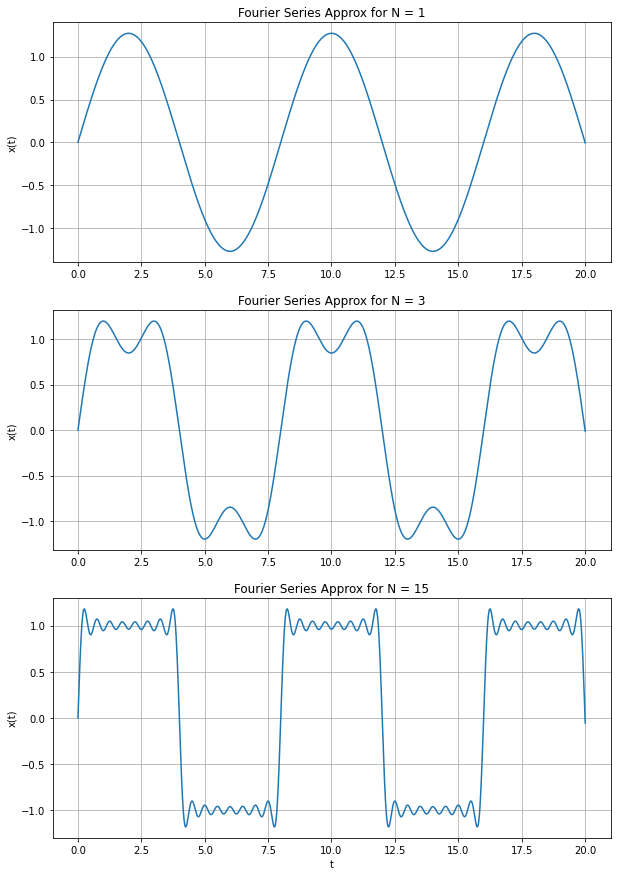
\includegraphics[scale=0.6]{fourier1.png}
    
    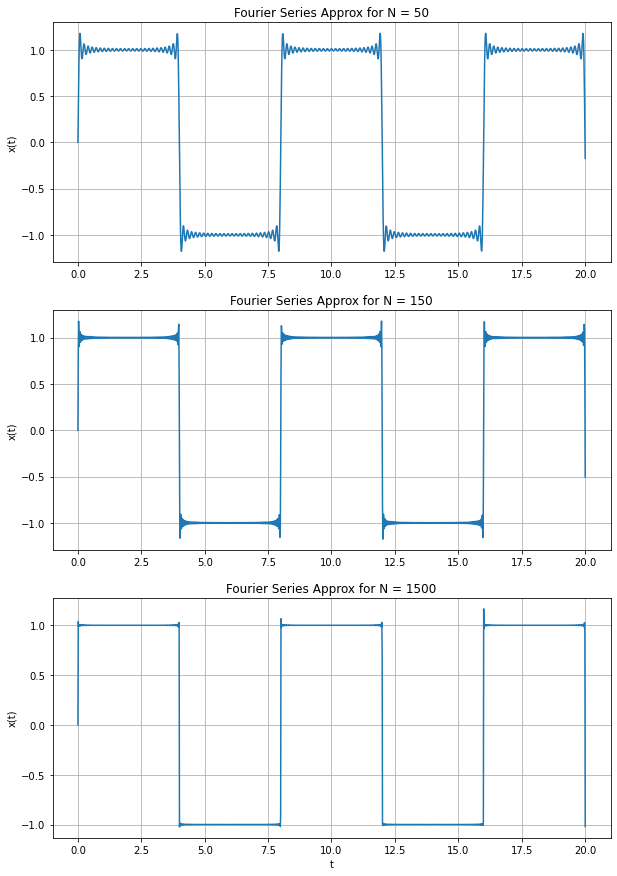
\includegraphics[scale=0.6]{fourier2.png}
    
    \paragraph{} As seen above, my expectations mostly held true. Although the approximation got better as N increased, the maximum N we tested wasn't good enough to make a perfect square wave for the human eye.  


\section{Error Analysis}

%This section will discuss error analysis of the experiment. Since this lab %deals with ideal simulation there shouldn't be any sources of error, so %instead this section can be used to describe any difficulties you had during %lab and how you solved them. Alternatively, if you couldn't get the %experiment to work, which is okay, you need to use this section to explain why %you couldn't get it to work to earn full points. 

\paragraph{} The main difficulty I encountered was conceptually grasping summation and how it applies to entire arrays. I'm still not used to being able to do operations on entire arrays at a single time. Python is a powerful tool I'm not yet adept in. I'm used to needing to iterate through each individual location like for C. So, changing my thought process into a fashion that takes advantage of Python's capabilities will be future for my future success in this lab. 

\paragraph{} As usual, a possible source of error is approximation. A large number of operations went into calculating just a single x(t). So, calculating a large number of them and summing those together is bound to have some degree of approximation.  

\section{Questions} %also address any deliverables not yet put in yet
    \begin{enumerate}
        \item  Is x(t) an even or an odd function? Explain why
        \paragraph{} It's an odd function, which explains why $a_k$ is normally zero since $a_k$ uses cosine which is an even function. It's an odd function because if you flip it over the x and y-axis, it's the same function.
        
        \item Based on your results from Task 1, what do you expect the values of $a_2$, $a_3$, ... , $a_n$ to be? Why?
        \paragraph{} I expect all of them to be zero since $a_k$ uses cosine which is an even function and x(t) is odd. We know cosine is even because it can be flipped over the x-axis, but not over the y-axis while still maintaining it's shape.
        
        \item How does the approximation of the square wave change as the value of N increases? In what way does the Fourier series struggle to approximate the square wave?
        \paragraph{} The approximation gets closer to an actual square wave as N increases. The Fourier series struggles to approximate the square wave, especially at the corner of the squares. As seen in the final plot within the "Results" section of my report, even at the number of sine waves at 1500, oscillations are visible when the square wave changes magnitude. 
                
        \item What is occurring mathematically in the Fourier series summation as the value of N increases?
        \paragraph{} More sinusoids are being used to generate the square wave, so it's shape is becoming closer to expected and more defined. Mathematically speaking, we're summing more values to calculate x(t), with the values being calculated through using increasingly more sine waves. 
                
        \item Leave any feedback on the clarity/usefulness of the purpose, deliverables, and expectations for this lab.
        \paragraph{} The goals of the lab, deliverables, and expectations were clear. 
    \end{enumerate}

\section{Conclusion}

%Discuss briefly what you learned in this lab and whether or not you feel the %lab was successful. Include any recommendations for future labs as this is a %learning experience for all of us. Discuss any insights you gained from this %lab and how that will affect future work. \textit{Note: The bibliograhpy %needs to be on its own page.}

    \paragraph{} During lab 8, I used Fourier Series to approximate periodic time-domain signals by taking advantage of symmetry for simplification  and loops for iteration. The lab was successful in introducing the students of Signals and Systems more to the concept of Fourier Transforms.   
    
    Github: \url{https://github.com/SethCram} 

\appendix

\chapter{Console Output}
    \begin{lstlisting}
        When k = 0 or 1, a_k =  0
        When k=1, b_k =  0.6366197723675814
        When k=2, b_k =  0.0
        When k=3, b_k =  0.2122065907891938
    \end{lstlisting}

\newpage

\end{document}